\documentclass{sciposter}
\usepackage{lipsum}
\usepackage{epsfig}
\usepackage{amsmath}
\usepackage{amssymb}
\usepackage{multicol}
\usepackage{graphicx,url}
\usepackage[portuges, brazil]{babel}   
\usepackage[utf8]{inputenc}
%\usepackage{fancybullets}
\newtheorem{Def}{Definition}

\title{wawa\\ Título provisório}
%Título do projeto

\author{Alexandre S. Bencz, Ezequiel F. Santos, Gabriel Fontenelle, Tales Pádua}
%nome dos autores

\institute 
{Bacharelado em Ciência da Computação\\
Centro Universitário SENAC - Campus Santo Amaro
  (SENAC-SP)\\
  Av. Engenheiro Eusébio Stevaux, 823 -- Santo Amaro, São Paulo -- CEP 04696-000 -- SP -- Brasil}
%Nome e endereço da Instituição

\email{{alebencz,ezefranca.br,colecionador.gabriel,talescpadua},{(@gmail.com})}
% Onde você coloca os emails dos integrantes


%\date is unused by the current \maketitle

\rightlogo[1]{Figures/UNAMiwi}
\leftlogo[1]{Figures/UNAMiwi}
% Exibe os logos (direita e esquerda) 
% Procure usar arquivos png ou jpg, e de preferencia mantenha na mesma pasta do .tex
%%%%%%%%%%%%%%%%%%%%%%%%%%%%%%%%%%%%%%%%%%%%%%%%%%%%%%%%%%%%%%%%%%%%%%%%%%%%%%%%
%%% Begin of Document

\begin{document}
%define conference poster is presented at (appears as footer)

\conference{{\bf E-COMP 2013}, 5º Encontro da Computação - Senac, 27 de Novembro de 2013, São Paulo, Brasil}

%\LEFTSIDEfootlogo  
% Uncomment to put footer logo on left side, and 
% conference name on right side of footer

% Some examples of caption control (remove % to check result)

%\renewcommand{\algorithmname}{Algoritme} % for Dutch

%\renewcommand{\mastercapstartstyle}[1]{\textit{\textbf{#1}}}
%\renewcommand{\algcapstartstyle}[1]{\textsc{\textbf{#1}}}
%\renewcommand{\algcapbodystyle}{\bfseries}
%\renewcommand{\thealgorithm}{\Roman{algorithm}}

\maketitle

%%% Begin of Multicols-Enviroment
\begin{multicols}{3}

%%% Abstract
\begin{abstract}
No modelo que a Danielle postou não tinha resumo, então confirmem para saber se precisa ou não.
Morphological pattern spectra computed from granulometries are frequently used
to classify the size classes of details in textures and images. An extension 
of this technique, which retains information on the spatial 
distribution of the details in each size class is developed. Algorithms for
computation of these spatial pattern spectra for a large number of 
granulometries on binary images are presented. 
\end{abstract}

%%% Introduction
\section{Introducão}
A importância do assunto deve ser destacada resumidamente.

\PARstart{G}{ranulometries} are ordered sets of morphological openings or closings, each of
which removes image details below a certain size. These can be used for texture
analysis
through the use of \emph{pattern spectra}, which show how the number of 
foreground pixels in the image changes as a function of the size parameter 
\cite{maragos89:_patter}.
A drawback of the classical definition of pattern spectra is that spatial 
information is not included in a pattern spectrum as shown below.
 In this paper, \emph{spatial pattern spectra} are developed which retain information on the distribution of these details at different scales.
 

\newcommand{\imsize}{0.45\columnwidth}
\begin{figure}
\begin{center}
\begin{tabular}{c c}

\end{tabular}
\end{center}
\caption{ Parts (a) through (c) show three images consisting of squares of
different sizes;
(d) shows the pattern spectra, denoting the number of foreground pixels 
 removed by openings by reconstruction by $\lambda \times \lambda$ squares. No 
granulometry is capable of separating the patterns, because the only 
differences between the images lie in the distributions of the 
connected components. }\label{fig:blocks}
\end{figure}




\section{Objetivos}
Dar uma ideia compacta da metodologia ou forma de abordagem da pesquisa, bem como o projeto foi desenvolvido.\\

Let binary images $X$ and $Y$ be defined as a subset of the image domain 
${\mathbf M}\subset {\mathbb Z}^n$ or ${\mathbb R}^n$ (usually $n=2$). 
\begin{Def}
A binary 
granulometry is a set of operators $\{\alpha_r\}$ with $r$ from some ordered 
set $\Lambda$ (usually $\Lambda \subset {\mathbb R}$ or ${\mathbb Z}$), with 
the following three properties
\begin{align}
   \alpha_r(X) & \subset  X \label{eq:antiext} \\
   X \subset Y & \Rightarrow \alpha_r(X) \subset \alpha_r(Y) 
   \label{eq:increasing} \\
   \alpha_r(\alpha_s(X)) & =  \alpha_{\max(r,s)}(X) \label{eq:idempot},
\end{align}   
for all $r,s \in \Lambda$.
\end{Def}

\begin{Def}
The pattern spectrum $s_{\alpha}(X)$ obtained by applying 
granulometry $\{\alpha_r\}$ to a binary image $X$ is defined as
\begin{equation}
    (s_{\alpha}(X))(u) = 
    - \frac{\partial A(\alpha_r(X))}{\partial r}\bigg{\vert}_{r=u}
\end{equation}
in which $A(X)$ is a function denoting the Lebesgue measure in 
${\mathbb R}^n$.
\end{Def} 
In the case of discrete images, and with $r \in \Lambda \subset {\mathbb Z}$, 
this differentiation reduces to
\begin{align}
    (s_{\alpha}(X))(r)  & = \#(\alpha_{r}(X) \setminus \alpha_{r^+}(X)) \\ 
                        & = \#(\alpha_{r}(X)) - \#(\alpha_{r^+}(X)), 
\end{align}
with $r^+ = \min\{ r' \in \Lambda \vert r' > r \}$, and $\#(X)$ the 
numnber of elements of $X$.

The opening transform \cite{Nacken:thesis} $\Omega_X$ of a binary image $X$ 
for a granulometry ${\alpha_r}$ is
\begin{equation}
  \Omega_X(x) = \max\{ r \in \Lambda \vert x \in \alpha_r(X) \}
\end{equation}

The pattern spectrum of a binary image $X$ using granulometry 
$\{\alpha_r\}$ is the histogram of $\Omega_X$ obtained with the same 
size distribution \cite{Nacken:thesis}, disregarding the bin for grey level 0.


\begin{figure}
\begin{center}
\end{center}
\caption{ \label{fig:opentransf} Opening transform with $\{\alpha_r\}$ as in 
 Fig. \ref{fig:blocks}: (left) original image; (right) opening transform
(contrast stretched for clarity). 
}
\end{figure}


\section{Metodologia}
Dar uma ideia compacta da metodologia ou forma de abordagem da pesquisa, bem como o projeto foi desenvolvido.
\\
Pattern spectra only retain the amount of detail present at  scale $r$.
This can be amended by computing some parameterization of the spatial 
distribution in an image $\alpha_r(X) \setminus \alpha_{r+}(X)$ as a function of $r$. 

\begin{Def}
Let ${M}(X)$ be some parameterization of the spatial distribution of detail
in the image $X$. The spatial pattern spectrum ${S}_{{M},\alpha}$ is
then defined as
\begin{equation}
  ({S}_{{M},\alpha}(X))(r) = {M}(\alpha_r(X) \setminus \alpha_{r+}(X)).
\end{equation}  
\end{Def}

An obvious parameterization of the spatial distribution is through 
the use of moments. Focusing on the case of 2-D binary images, the 
moment $m_{ij}$ of order $ij$ of an image $X$ is given by
\begin{equation}
  m_{ij}(X) = \sum_{(x,y) \in \mathbf X} x^i y^j.
\end{equation}  
The spatial moment spectrum $S_{m_{ij},\alpha}$ of order $ij$ is
\begin{equation}
  (S_{m_{ij},\alpha}(X))(r) = m_{i,j}(\alpha_r(X) \setminus \alpha_{r^+}(X)).
\end{equation}  
For $i=0$ and $j=0$ we obtain the standard pattern spectrum. 
For each $r$, $(S_{m_{ij},\alpha}(X))(r)$ is just the moment of an image, 
therefore, derived parameters such as coordinates of the centre of mass, 
(co-)variances, skewness and kurtosis of the distribution of details at each
scale can be computed easily. We can then define pattern mean
spectra, pattern (co-)variance spectra, pattern kurtosis spectra, etc. The 
pattern mean-$x$ and variance-$x$ spectra 
($S_{\bar x,\alpha}$ and $S_{\sigma(x),\alpha}$) are defined as: 
\begin{align}
  S_{\bar x,\alpha} & = \frac{S_{m_{10},\alpha}} {S_{m_{00},\alpha}} \\
\intertext{and}
   S_{\sigma(x),\alpha} & = \sqrt{\frac{S_{m_{20},\alpha}}
                                 {S_{m_{00},\alpha}} 
                                 - S_{\bar x, \alpha}}.  
 \end{align}
These two are shown in Figures \ref{fig:tauspect} and \ref{fig:binspect}. Note that 
these definitions hold only where $(S_{m_{00},\alpha}(f))(r) \neq 0$. For all 
other values of $r$ they will be defined as zero. Further post-processing can
be done to compute central moments and moment invariant from pattern moment 
spectra \cite{Flusser:Suk:93,Hu:62}. 

\section{Resultados e Discussão}

Verificar os principais resultados obtidos de acordo com os objetivos propostos.\\

Nacken \cite{Nacken:thesis} derived an algorithm for computation
of pattern spectra for granulometries based on openings by discs of increasing
radius for various metrics, using the opening transform. After the
opening transform has been computed, it is straightforward to compute the 
pattern spectrum:
\begin{itemize}
\item Set all elements of array {\tt S} to zero
\item For all $x \in X$ increment {\tt S}[$\Omega_X(x)$] by one. 
\end{itemize}

To compute the pattern \emph{moment} spectrum, the only thing that needs to be
changed is the way {\tt S}[$\Omega_X(x)$] is incremented. As shown in Algorithm
\ref{alg:spect}.

\begin{algorithm}
\begin{itemize}
\item Set all elements of array {\tt S} to zero
\item For all $(x,y) \in X$ increment {\tt S}[$\Omega_X(x,y)$] by 
$x^iy^j$. 
\end{itemize}
\caption{ Algorithm for computation of pattern moment
spectrum of order $ij$. \label{alg:spect}}
\end{algorithm}

This algorithm can 
readily be adapted to other granulometries, simply by computing the 
appropriate opening transform.

\begin{figure}
\begin{center}
\begin{tabular}{c c}

\end{tabular}
\end{center}
\caption{ \label{fig:tauspect} 
The opening transform using city-block metric: (a) opening transform of
Fig. 1(c); (b) pattern spectrum; (c) pattern variance-$x$; 
(d) variance-$y$ spectra.}
\end{figure}


\renewcommand{\imsize}{0.3\columnwidth}
\begin{figure}
\begin{center}
\end{center}
\caption{ \label{fig:binspect} Pattern mean-$x$ (top) and variance-$x$ 
(bottom) spectra: the three collumns show spectra for Fig. 1(a), (b) and (c) 
from left to right respectively.  Unlike the standard pattern spectra, 
these spatial pattern spectra can distinguish the three images.}
\end{figure}

\section{Conclusão}

Sitting on a corner all alone,
staring from the bottom of his soul,
watching the night come in from the window

\begin{figure}
\centering
\includegraphics[width=0.7\textwidth]{Figures/Diff_Dprime.eps}
\end{figure}
\\
It'll all collapse tonight, the fullmoon is here again
In sickness and in health, understanding so demanding
It has no name, there's one for every season
Makes him insane to know
\\
Running away from it all
"I'll be safe in the cornfields", he thinks
Hunted by his own,
again he feels the moon rising on the sky
\\
Find a barn which to sleep in, but can he hide anymore
Someone's at the door, understanding too demanding
Can this be wrong, it's love that is not ending
Makes him insane to know
\\
She should not lock the open door
(Run away, run away, run away)
Fullmoon is on the sky and He's not a man anymore
sees the change in him but can't
(Run away, run away, run away)
See what became out of her man
Fullmoon
\\
Swimming across the bay,
the night is gray, so calm today
She doesn't wanna wait.
"We've gotta make the love complete tonight..."
\\
In the mist of the morning he cannot fight anymore
Hundred moons or more, he's been howling
Knock on the door, and scream that is soon ending
Mess on the floor again
\\
She should not lock the open door
(Run away, run away, run away)
Fullmoon is on the sky and he's not a man anymore
She sees the changes in him but can't
(Run away, run away, run away)
See what became out of her man
\\
She should not lock the open door
(Run away, run away, run away)
Fullmoon is on the sky and he's not a man anymore
sees the changes in him but can't
(Run away, run away, run away)
See what became out of her darling man
\\
She should not lock the open door
(Run away, run away, run away)
Fullmoon is on the sky and he's not a man anymore
See what became out of her man
 
%%% References

%% Note: use of BibTeX als works!!

\bibliographystyle{plain}
\begin{thebibliography}{1}

\bibitem{Flusser:Suk:93}
J.~Flusser and T.~Suk.
\newblock Pattern recognition by affine moment invariants.
\newblock {\em Pattern Recognition}, 26:167--174, 1993.

\bibitem{Hu:62}
M.~K. Hu.
\newblock Visual pattern recognition by moment invariants.
\newblock {\em IRE Transactions on Information Theory}, IT-8:179--187, 1962.

\bibitem{maragos89:_patter}
P.~Maragos.
\newblock Pattern spectrum and multiscale shape representation.
\newblock {\em IEEE Trans. Patt. Anal. Mach. Intell.}, 11:701--715, 1989.

\bibitem{Meijster:Wilkinson:PAMI}
A.~Meijster and M.~H.~F. Wilkinson.
\newblock A comparison of algorithms for connected set openings and closings.
\newblock {\em IEEE Trans. Patt. Anal. Mach. Intell.}, 24(4):484--494, 2002.

\bibitem{Nacken:thesis}
P.~F.~M. Nacken.
\newblock {\em Image Analysis Methods Based on Hierarchies of Graphs and
  Multi-Scale Mathematical Morphology}.
\newblock PhD thesis, University of Amsterdam, Amsterdam, The Netherlands,
  1994.

\end{thebibliography}

\end{multicols}

\end{document}